\section{Background}
\label{sec:background}

\begin{figure}[t]
	%\vskip 0.2in
	\begin{center}
		\centerline{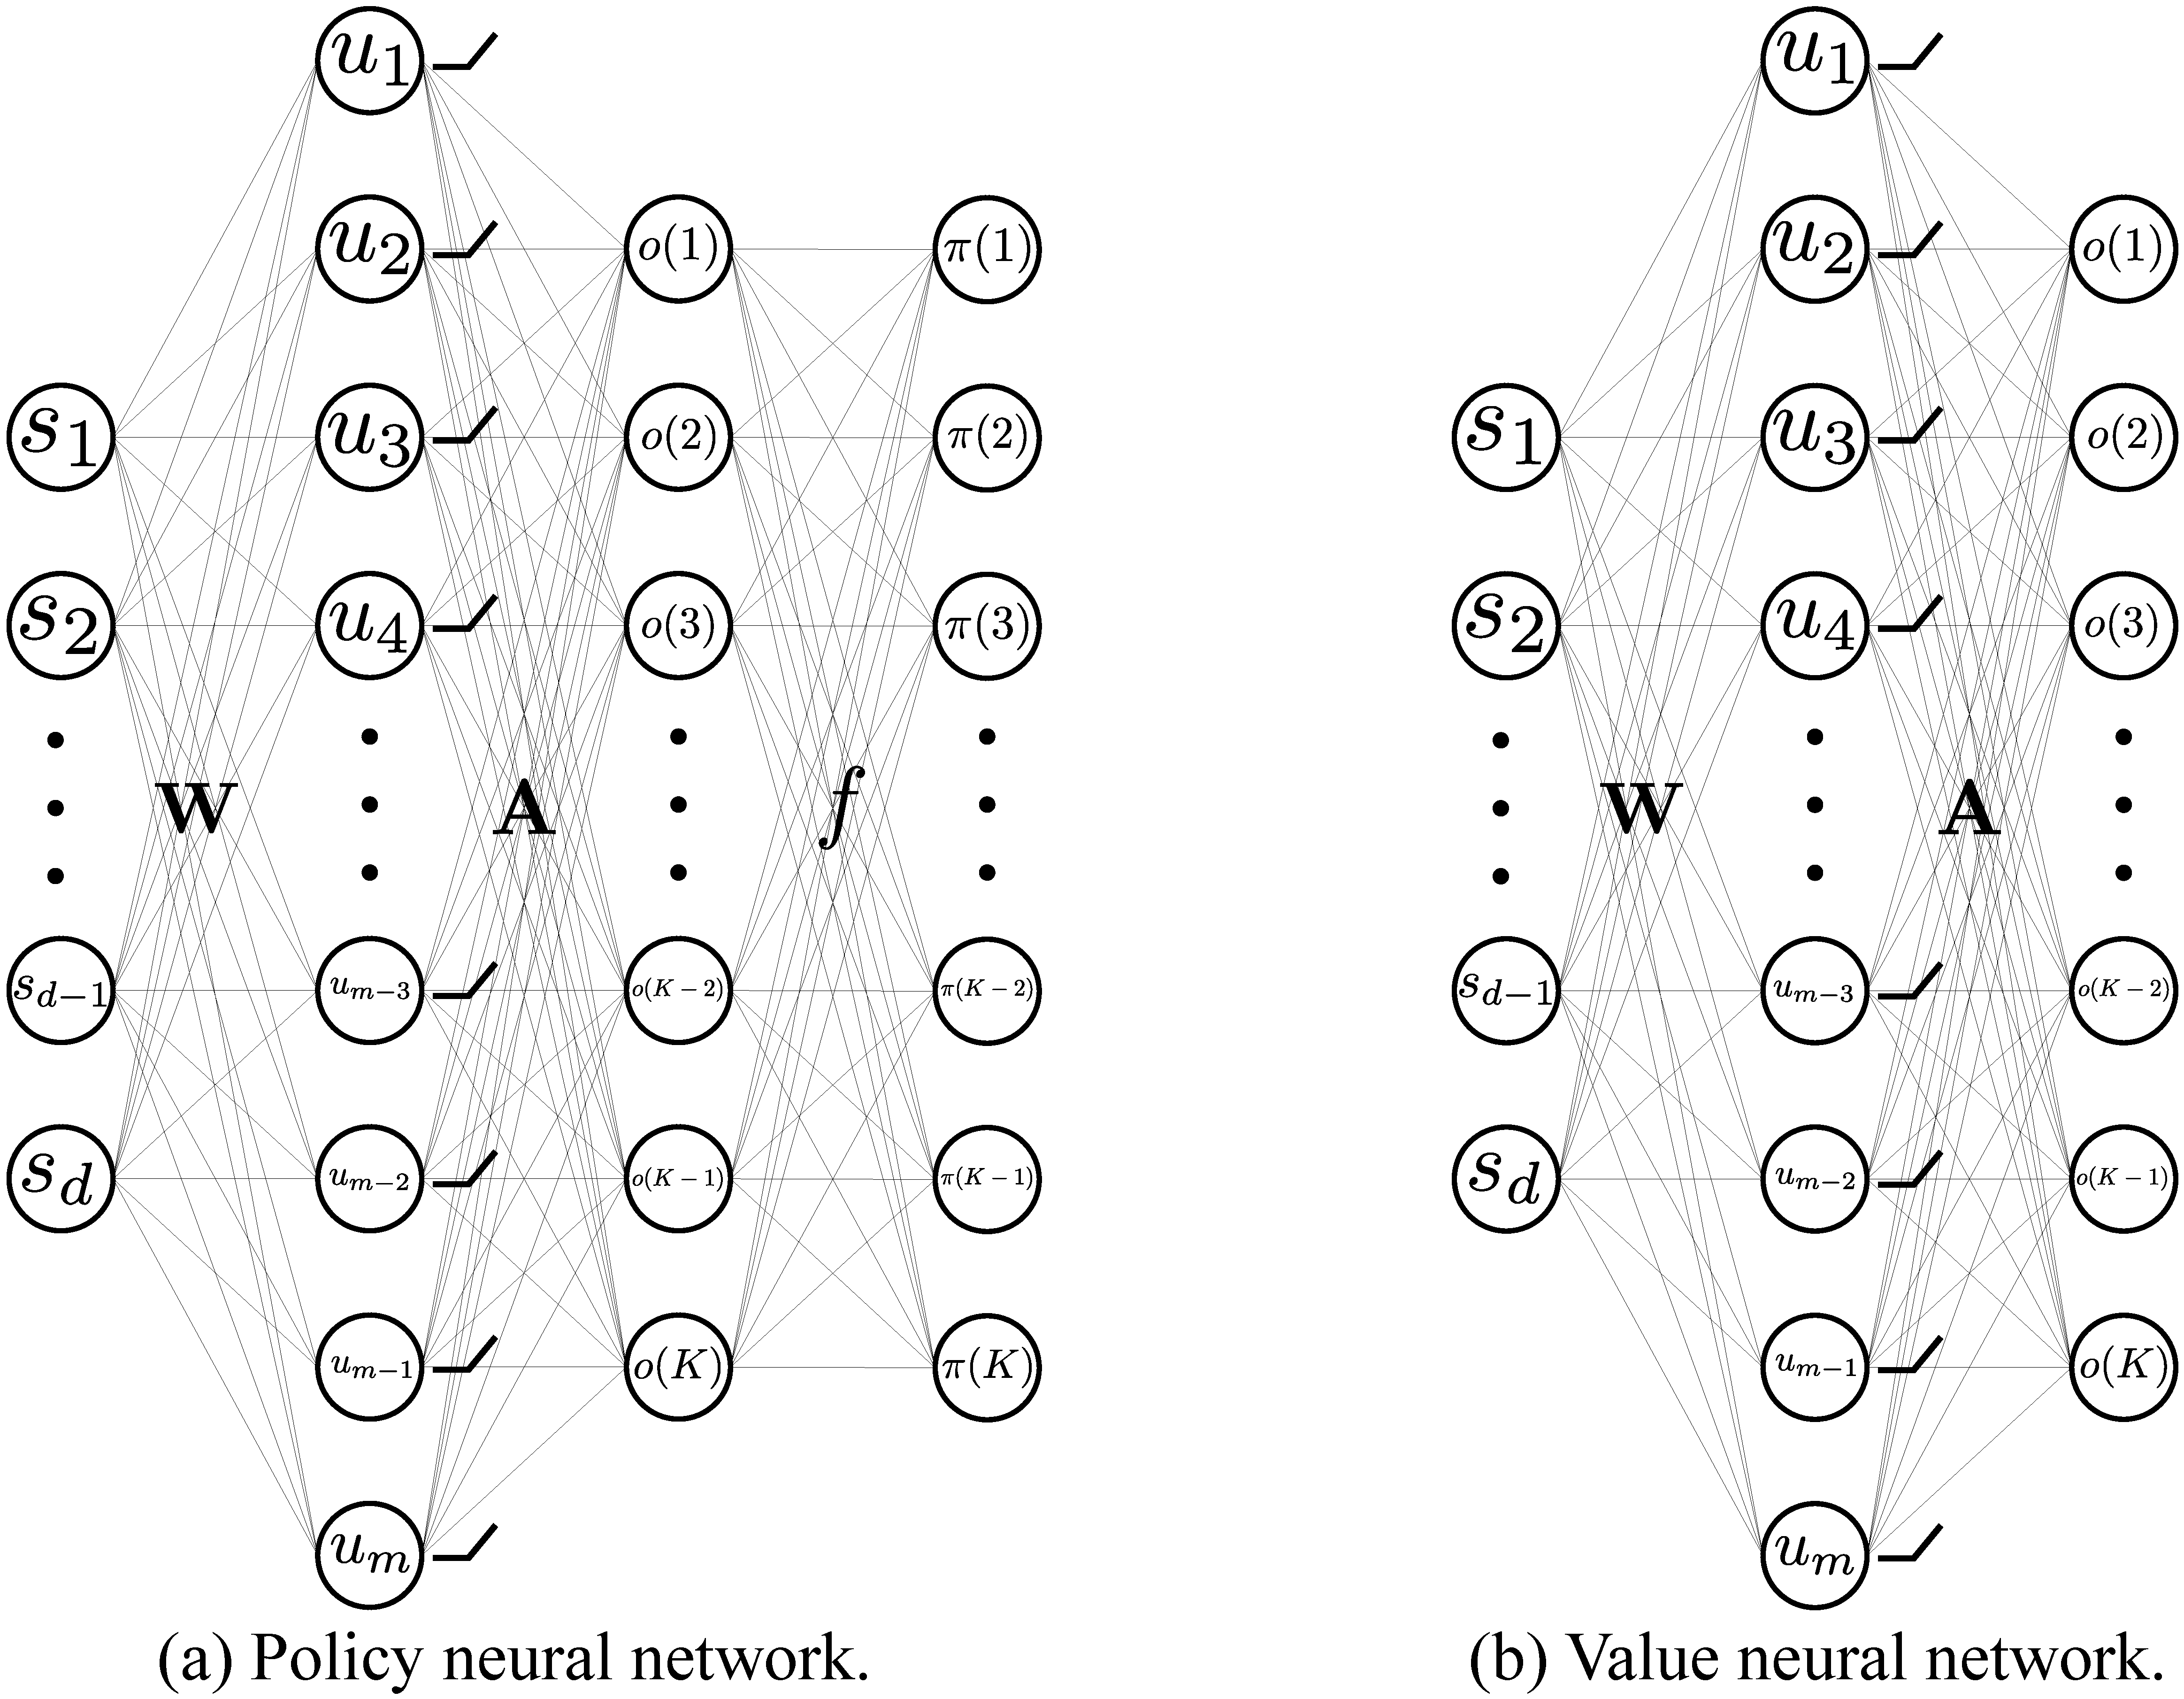
\includegraphics[width=1.0\columnwidth]{nn_policy_value_vertical_aistats.pdf}}
		\caption{The structure of policy neural network and value neural network.}
		\label{fig:nn_policy_value}
	\end{center}
	\vskip -0.2in
\end{figure}

We mainly focus on the stochastic bandit setting in this paper, where the policy or action values are represented using a two-layer neural network.  
The results can be generalized to other reinforcement learning settings, such as and episodic MDPs and contextual bandits; further discussion will be provided in \cref{sec:general_settings}.

\subsection{Stochastic Multi-Armed Bandit (MAB)}
\label{subsec:settings}

One can consider the standard stochastic MAB setting to only have one state, i.e., $n=1$.  
%At each time step $t$, the agent takes an action $A_t \in [h]$ according to its own strategies $\rvpi_t$, and then it observes a random reward $R\left(A_t\right) \in \sR$, where the mean value of $R\left(A_t\right)$ is $r\left(A_t\right)$. 
%The agent then improves its action selection strategies. 
After $T$ time steps, the performance of the agent's strategy is measured by the (expected) regret,
\begin{equation}
\label{eq:expected_regret}
\scalemath{0.85}{
R_T = \sum\limits_{t=0}^{T-1}{{\rvpi^*}^\top \rvr} - \sE \left[ \sum\limits_{t=0}^{T-1}{  r\left(A_t\right)  } \right] = \sum_{t=0}^{T-1} \sum_k \pi_t(k) \Delta(k).
%= \sum\limits_{t=0}^{T-1}{{\rvpi^*}^\top \rvr} - \sum\limits_{t=0}^{T-1}{ \sE \left[ r\left(A_t\right) \right] },
}
\end{equation}
where the expectation is over the randomness of action selection, if the agent is using stochastic strategies. In the second equality, $\rvpi^*$ is a one-hot vector, $\Delta(a) = \max_{k^\prime} r(k^\prime)- r(k)$, and  $r(k)$ is the true mean reward of action $k$.
Without loss of generality, we assume $\rvr \in \left[ 0, 1 \right]^K$ in this paper.

%\subsubsection{Episodic Markov decision process (MDP) (maybe remove this section)}
%The episodic MDP setting recovers the bandit setting as a special case. The environment randomly select a starting state $\rvs_i^0 \in \sR^d$. At each time step $t$, the agent takes one action $A_t \in [h]$ according to some strategies, and then it observes a reward $R_{i, A_t} \in \sR$ and next state $S_{t+1} \sim \sP\left( \cdot \middle| S_t, A_t \right)$, where $\sP$ is the transition probability matrix and it is unknown to the agent. After such $H$ steps, the agent observes an ending state $S_H$, and the current trajectory terminates. At the next time step, the agent will observe a new starting state $\rvs_i^0$ randomly generated by the environment. Since we use policy gradient method (no value learning), the agent updates its neural network policy weights using the cumulative reward collected after each single trajectory terminates.

%We mainly focus on the standard stochastic bandit setting with $n = 1$, i.e., there is only one state $\rvs_i$. At each time step $t$, the agent takes an action $A_t \in [h]$ according to its own strategies, and then it observes a random reward $R_{i, A_t} \in \sR$, where the mean value of $R_{i, A_t}$ is $r_{i, A_t}$. The agent then uses the reward to improve its action selection strategies. After such $T$ time steps, the performance of the agent's strategy is measured by the (expected) regret,
%\begin{equation}
%\label{eq:expected_regret}
%    \sum\limits_{t=0}^{T-1}{{\rvpi_i^*}^\top \rvr_i} - \sE \left[ \sum\limits_{t=0}^{T-1}{  r_{i, A_t}  } \right] = \sum\limits_{t=0}^{T-1}{{\rvpi_i^*}^\top \rvr_i} - \sum\limits_{t=0}^{T-1}{ \sE \left[ r_{i, A_t} \right] },
%\end{equation}
%where the expectation is over the randomness of action selection, if the agent is using some stochastic strategies.

\subsection{Policy- and Value-based RL Methods}

Minimizing the regret \cref{eq:expected_regret} is usually formulated as a policy optimization problem, i.e., $\max\limits_{\rvpi \in \Pi}{ \expectation\limits_{ k \sim \rvpi }{ r(k)} }$, where $\Pi$ is the policy constraint. In practice, when $\Pi$ consists of all $\rvpi(\rmW)$ represented by the parameter $\rmW$, one can use iterative gradient updates to solve the expected reward maximization problem. This is known as the policy gradient method.

On the other hand, value based RL methods directly learn a function to approximate the value/logit of the optimal policy, i.e., $\min\limits_{\rvo \in \gO}{ \expectation\limits_{k \sim \rvb}{ \left\| o(k) - o^*(k) \right\|^2 }}$, where $\rvb$ is a behavior policy that samples actions for learning. The learned value function induces a policy that acts greedily with respect to the value of each action.

\subsection{Neural Networks as Policy/Value Function Approximations}
\label{subsec:nn_value_policy}
 

%Both the value and the policy neural networks take the state feature  $\rvs_i \in \sR^d$ as the input. Then the networks calculate the hidden node value vector by $u_{i,r} \triangleq \rvw_r^\top \rvs_i$, $\forall r \in [m]$. The logit vector is then calculated by $o_{i,k} \triangleq \rva_k^\top \sigma\left( \rvu_i \right)$, $\forall k \in [h]$, where $\sigma$ is element-wise ReLU activation function. The value neural network outputs the logit vector $\rvo_i$. While the policy neural network output probability is the softmax transform of the logit vector, i.e., $\rvpi_i \triangleq f\left( \rvo_i \right) = f\left( \rmA \sigma\left( \rmW \rvs_i \right) \right)$. 

%The policy neural network defines a family of policies $\rvpi_i \left( \rmW \right)$ parameterized by $\rmW \in \sR^{m \times d}$ given any state $\rvs_i$. Let $\rvpi_i = \rvpi_i \left( \rmW \right)$, the expected loss of the policy neural network can be calculated according to \cref{eq:expected_loss}.

%\paragraph{Initialization of the matrix $\rmA$.} 
We assume that the networks have the state $\rvs$ as input, satisfying $\left\| \rvs \right\|_2 = 1$.
As can be seen later, our algorithm randomly initializes the weight matrix $\rmA$ and fixes it during learning. 
This is a common strategy when using over-parametrized neural networks \citep{li2018learning,du2018gradientA,du2018gradientB,allen2018convergenceA,allen2018convergenceB}, and it has been verified empirically that there is no impact on the performance of trained neural networks \citep{hoffer2018fix}.
In this paper, each element in $\rmA$ is initialized by $a_{k,r} \sim \unif\left\{-1, +1\right\}$. Other initializations, such as $\rva_k \sim \gN(0, \rmI)$ will also work. In rest of the paper, we denote the policy $\rvpi(\rmW_t)$ by $\rvpi_t$ for simplicity.
%\paragraph{Multi-layered neural networks.} 

The proposed algorithms and results can be extended to general value functions and policies parametrized by multi-layered neural networks, by resorting to related techniques \citep{allen2018convergenceA,allen2018convergenceB,du2018gradientA}. For the sake of simplicity and conciseness, we focus only on two-layer neural networks in the paper.

%Although there is only one state, i.e., $n = 1$, and $i$ can be omitted without ambiguity, we choose to keep the subscript $i$ here to make the generalization from the standard bandit setting to the many state dependent setting smoother, and our algorithms work for general $n > 1$. For simplicity, we assume $\left\| \rvs_{i} \right\|_2 = 1$, $\forall i \in [n]$.

%In the case of $n > 1$, for each state $\rvs_i$, there is a state dependent policy $\rvpi_i$. And the agent's goal is to learn totally $n$ policies using only one neural network. We assume $\left\| \rvs_{i} -  \rvs_{j} \right\|_2 \ge \delta > 0 , \ \forall i \not= j$, i.e., no duplicated data, and $\left\| \rvs_{i} \right\|_2 = 1, \ \forall i \in [n]$.
